\achapter{23}{The Dot Product in $\R^n$} \label{sec:dot_product}

\vspace*{-17 pt}
\framebox{
\parbox{\dimexpr\linewidth-3\fboxsep-3\fboxrule}
{\begin{fqs}
\item What is the dot product of two vectors? Under what conditions is the dot product defined? 
\item How do we find the angle between two nonzero vectors in $\R^n$?
\item How does the dot product tell us if two vectors are orthogonal? 
\item How do we define the length of a vector in any dimension and how can the dot product be used to calculate the length? 
\item How do we define the distance between two vectors? 
\item What is the orthogonal projection of a vector $\vu$ in the direction of the vector $\vv$ and how do we find it? 
\item What is the orthogonal complement of a subspace $W$ of $\R^n$? 
\end{fqs}}}% \hspace*{3 pt}}

\vspace*{13 pt}

\csection{Application: Hidden Figures in Computer Graphics}

 In video games, the speed at which a computer can render changing graphics views is vitally important. To increase a computer's ability to render a scene, programs often try to identify those parts of the images a viewer could see and those parts the viewer could not see. For example, in a scene involving buildings, the viewer could not see any images blocked by a solid building. In the mathematical world, this can be visualized by graphing surfaces. In  Figure \ref{F:House} we see a crude image of a house made up of small polygons (this is how programs generally represent surfaces). On the left in Figure \ref{F:House} we see all of the polygons that are needed to construct the entire surface, even those polygons that lie behind others which we could not see if the surface was solid. On the right in Figure \ref{F:House} we have hidden the parts of the polygons that we cannot see from our view. 
 \begin{figure}[ht] 
\begin{center}
\resizebox{!}{1.5in}{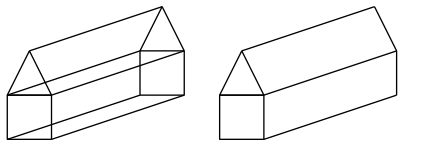
\includegraphics{6_a_House}}
\caption{Images of a house.}
\label{F:House}
\end{center}
\end{figure}
We also see this idea in mathematics when we graph surfaces. Figure \ref{F:Surface} shows the graph of the surface defined by $f(x,y) = \sqrt{4-x^2}$ that is made up of polygons. At left we see all of the polygons and at right only those parts that would be visible from our viewing perspective. 
\begin{figure}[h]
\begin{center}
\resizebox{!}{2.0in}{\includegraphics{6_a_Surface_1.eps}} \hspace{0.1in} \resizebox{!}{2.0in}{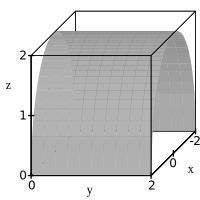
\includegraphics{6_a_Surface_2.eps}}
\end{center}
\caption{Graphs of $f(x,y) = \sqrt{4-x^2}$.}
\label{F:Surface}
\end{figure}
By eliminating the parts of the polygons we cannot see from our viewing perspective, the computer program can more quickly render the viewing image. Later in this section we will explore one method for how programs remove the hidden portions of images. This process involves the dot product of vectors.  

\csection{Introduction}

Orthogonality, a concept which generalizes the idea of perpendicularity, is an important concept in linear algebra. We use the dot product to define orthogonality and more generally angles between vectors in $\R^n$ for any dimension $n$. The dot product has many applications, e.g., finding components of forces acting in different directions in physics and engineering. The dot product is also an example of a larger concept, \emph{inner products}, that we will discuss later. We introduce and investigate dot products in this section.

We will illustrate the dot product in $\R^2$, but the process we go through will translate to any dimension. Recall that we can represent the vector $\vv = \left[ \begin{array}{c} v_1 \\ v_2 \end{array} \right]$ as the directed line segment (or arrow) from the origin to the point $(v_1, v_2)$ in $\R^2$, as illustrated in Figure \ref{F:6_a_Vector_norm}. Using the Pythagorean Theorem we can then define the length (or magnitude or norm) of the vector $\vv$ in $\R^2$ as
\[|| \vv || = \sqrt{v_1^2 + v_2^2}.\]
We can also write this norm as
\[\sqrt{v_1v_1 + v_2v_2}.\]
The expression under the square root is an important one and we extend it and give it a special name.
\begin{figure}[ht] \centering
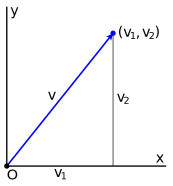
\includegraphics[width=3.7cm]{6_a_Vector_norm}
\caption{A vector in $\R^2$ from the origin to a point.}
\label{F:6_a_Vector_norm}
\end{figure}

If $\vu = [ u_1 \ u_2 ]^{\tr}$ and $\vv = [ v_1 \ v_2]^{\tr}$ are vectors in $\R^2$, then we call the expression $u_1v_1+u_2v_2$ the \emph{dot product} of $\vu$ and $\vv$, and denote it as $\vu \cdot \vv$. With this idea in mind, we can rewrite the norm of the vector $\vv$ as
\[|| \vv || = \sqrt{\vv \cdot \vv}.\]

The definition of the dot product translates naturally to $\R^n$ (see Exercise \ref{ex:1_e_scalar_product} in Section \ref{sec:matrix_vector}).

\begin{definition} \label{def:6_a_dot_product} Let $\vu = [u_1 \ u_2 \ \cdots \ u_n]$ and $\vv = [ v_1 \ v_2 \ \cdots \ v_n ]$ be vectors in $\R^n$. The \textbf{dot product}\index{dot product} (or \textbf{scalar product}\index{scalar product}) of $\vu$ and $\vv$ is the scalar
\[\vu \cdot \vv = u_1v_1 + u_2v_2 + \cdots + u_nv_n = \displaystyle \sum_{i=1}^n u_iv_i.\]
\end{definition}

The dot product then allows us to define the norm (or magnitude or length) of any vector in $\R^n$.

\begin{definition} \label{def:6_a_length_Rn} The \textbf{norm}\index{vector!norm in $\R^n$} $||\vv||$ of the vector $\vv \in \R^n$ is 
\[||\vv|| = \sqrt{\vv \cdot \vv}.\]
\end{definition}

We also use the words \textbf{magnitude}\index{vector!magnitude in $\R^n$} or \textbf{length}\index{vector!length in $\R^n$} as alternatives for the word norm. We can equivalently write the norm of the vector $\vv = [ v_1 \ v_2 \ \cdots \ v_n ]^{\tr}$ as 
\[||\vv|| = \sqrt{v_1^2 + v_2^2 + \cdots + v_n^2}.\]

We can also realize the dot product as a matrix product. If $\vu = [ u_1 \ u_2 \ \cdots \ u_n ]^{\tr}$ and $\vv = [  v_1 \ v_2 \ \cdots \ v_n ]^{\tr}$, then
\[\vu \cdot \vv = \vu^{\tr}\vv.\footnote{Technically, $\vu^{\tr}\vv$ is a $1 \times 1$ matrix and not a scalar, but we usually think of $1 \times 1$ matrices as scalars.}\]

\noindent \textbf{IMPORTANT NOTE: } The dot product is only defined between two vectors with the \emph{same number of components}.


\begin{pa} \label{pa:6_a} ~
\be
\item Find $\vu \cdot \vv$ if $\vu = [2 \ 3 \ -1 \ 4]^{\tr}$ and $\vv = [4 \ 6 \ 7 \ -5]^{\tr}$ in $\R^4$.


\item The dot product satisfies some useful properties as given in the next theorem.

\begin{theorem} \label{thm:6_a_dot_product} Let $\vu$, $\vv$, and $\vw$ be vectors in $\R^n$, and let $c$ be a scalar. Then
\ba
\item $\vu \cdot \vv = \vv \cdot \vu$ (the dot product is \emph{commutative}),
\item $(\vu + \vv) \cdot \vw = (\vu \cdot \vw) + (\vv \cdot \vw)$ (the dot product \emph{distributes over vector addition}),
\item $(c\vu) \cdot \vv = \vu \cdot (c\vv) = c(\vu \cdot \vv)$,
\item $\vu \cdot \vu \geq 0$ with equality if and only if $\vu = \vzero$,
\item $||c \vu || = |c| ||\vu||$.  
\ea
\end{theorem}

Verification of some of these properties is left to the exercises.  Let $\vu$ and $\vv$ be vectors in $\R^5$ with $\vu \cdot \vv = -1$, $|| \vu || = 2$ and $|| \vv || = 3$. 
    \ba
    \item Use property (c) of Theorem \ref{thm:6_a_dot_product} to determine the value of $\vu \cdot 2\vv$.

    \item Use property (b) of Theorem \ref{thm:6_a_dot_product} to determine the value of $(\vu + \vv) \cdot \vv$.

    \item Use whatever properties of Theorem \ref{thm:6_a_dot_product} that are needed to determine the value of $(2\vu+4\vv) \cdot (\vu - 7\vv)$.

	\ea
	
\item At times we will want to find vectors in the direction of a given vector that have a certain magnitude. Let $\vu = [2 \ 2 \ 1]^{\tr}$ in $\R^3$.
	\ba
	\item What is $|| \vu ||$? 

	\item Show that $\left| \left| \frac{1}{||\vu||} \vu \right| \right| = 1$. 

	
	\item Vectors with magnitude 1 are important and are given a special name.

\begin{definition} \label{def:6_a_unit_vector} A vector $\vv$ in $\R^n$ is a \textbf{unit vector}\index{unit vector} if $|| \vv || = 1$.
\end{definition}

We can use unit vectors to find vectors of a given length in the direction of a given vector. Let $c$ be a positive scalar and $\vv$ a vector in $\R^n$. Use properties from Theorem \ref{thm:6_a_dot_product} to show that the magnitude of the vector $c \frac{\vv}{||\vv||}$ is $c$. 

	\ea
		

\ee

\end{pa}


\csection{The Distance Between Vectors}

Finding optimal solutions to systems is an important problem in applied mathematics. It is often the case that we cannot find an exact solution that satisfies certain constraints, so we look instead for the ``best" solution that satisfies the constraints. An example of this is fitting a least squares line to a set of data. As we will see, the dot product will allow us to find ``best" solutions to certain types of problems, where we measure accuracy using the notion of a distance between vectors. Geometrically, we can represent a vector $\vu$ as a directed line segment from the origin to the point defined by $\vu$. If we have two vectors $\vu$ and $\vv$, we can think of the length of the difference $\vu - \vv$ as a measure of how far apart the two vectors are from each other. It is natural, then to define the distance between vectors as follows.

\begin{definition} \label{def:6_a_distance} Let $\vu$ and $\vv$ be vectors in $\R^n$. The \textbf{distance}\index{distance between vectors} between $\vu$ and $\vv$ is the length of the difference $\vu - \vv$ or
\[|| \vu - \vv ||.\]
\end{definition}


As Figure \ref{F:6_a_vector_difference} illustrates, if vectors $\vu$ and $\vv$ emanate from the same initial point, and $P$ and $Q$ are the terminal points of $\vu$ and $\vv$, respectively, then the difference $|| \vu - \vv||$  is the standard Euclidean distance between the points $P$ and $Q$. 
\begin{figure}[ht] \centering
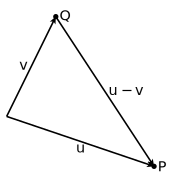
\includegraphics[width=3.7cm]{6_a_vector_difference}
\caption{$|| \vu - \vv||$.}
\label{F:6_a_vector_difference}
\end{figure}



\csection{The Angle Between Two Vectors}

Determining a ``best" solution to a problem often involves finding a solution that minimizes a distance. We generally accomplish a minimization through orthogonality --  which depends on the angle between vectors. Given two vectors $\vu$ and $\vv$ in $\R^n$, we position the vectors so that they emanate from the same initial point. If the vectors are nonzero, then they determine a plane in $\R^n$. In that plane there are two angles that these vectors create. We will define the angle between the vectors to be the smaller of these two angles. The dot product will tell us how to find the angle between vectors. Let $\vu$ and $\vv$ be vectors in $\R^n$ and $\theta$ the angle between them as illustrated in Figure \ref{F:Angle}.
\begin{figure}[h]
\begin{center}
\resizebox{!}{1.5in}{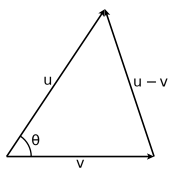
\includegraphics{6_a_Angle.eps}}
\end{center}
\caption{The angle between $\vu$ and $\vv$}
\label{F:Angle}
\end{figure}
Using the Law of Cosines, we have
\[ ||\vu-\vv||^2=||\vu||^2+||\vv||^2 - 2||\vu|| \ ||\vv|| \ \cos(\theta) \,.\]
Rearranging, we obtain 
\begin{align*}
||\vu|| \ ||\vv|| \ \cos(\theta) &= \frac{1}{2} \left( ||\vu||^2+||\vv||^2 - ||\vu-\vv||^2 \right) \\
&= \frac{1}{2} (||\vu||^2+||\vv||^2 - (\vu-\vv)\cdot (\vu-\vv) )\\
&= \frac{1}{2} (||\vu||^2+||\vv||^2 - \vu\cdot \vu +2\vu \cdot \vv - \vv\cdot \vv ) \\
&= \vu \cdot \vv  \, .
\end{align*}
%\begin{align*}
%|| \vu - \vv ||^2 &= ||\vu||^2 + ||\vv||^2 - 2||\vu|| \ ||\vv|| \ \cos(\theta) \\
%(\vu - \vv) \cdot (\vu - \vv)  &= ||\vu||^2 + ||\vv||^2 - 2||\vu|| \ ||\vv|| \ \cos(\theta) \\
%(\vu \cdot \vu) - 2 (\vu \cdot \vv) + (\vv \cdot \vv) &= ||\vu||^2 + ||\vv||^2 - 2||\vu|| \ ||\vv|| \ \cos(\theta) \\
%||\vu||^2 - 2 (\vu \cdot \vv) + ||\vv||^2 &= ||\vu||^2 + ||\vv||^2 - 2||\vu|| \ ||\vv|| \ \cos(\theta) \\
%- 2 (\vu \cdot \vv)  &= - 2 \ ||\vu|| \ ||\vv|| \ \cos(\theta) \\
%\vu \cdot \vv  &= ||\vu|| \ ||\vv|| \ \cos(\theta).
%\end{align*}
So the angle $\theta$ between two nonzero vectors $\vu$ and $\vv$ in $\R^n$ satisfies the equation
\begin{equation} \label{eq:6_a_angle_between}\index{angle between vectors} 
\cos(\theta) = \frac{\vu \cdot \vv}{||\vu|| \ ||\vv||}.
\end{equation}

Of particular interest to us will be the situation where vectors $\vu$ and $\vv$ are \emph{orthogonal} (perpendicular).\footnote{We use the term orthogonal instead of perpendicular because we will be able to extend this idea to situations where we normally don't think of objects as being perpendicular.} Intuitively, we think of two vectors as orthogonal if the angle between them is $90^{\circ}$. 



\begin{activity} \label{act:6_a_orthogonality} ~ 
	\ba
	\item The vectors $\ve_1 = [ 1 \ 0]^{\tr}$ and $\ve_2 = [0 \ 1]^{\tr}$ are perpendicular in $\R^2$. What is $\ve_1 \cdot \ve_2$?
	
	
	
	\item Now let $\vu$ and $\vv$ be any vectors in $\R^n$. 
		\begin{enumerate}[i.]
		\item Suppose the angle between nonzero vectors $\vu$ and $\vv$ is $90^{\circ}$. What does Equation (\ref{eq:6_a_angle_between}) tell us about $\vu \cdot \vv$?
		
		
		
		\item Now suppose that $\vu \cdot \vv = 0$. What does Equation (\ref{eq:6_a_angle_between}) tell us about the angle between $\vu$ and $\vv$? Why?
		
		
		
		\item Explain why the following definition makes sense.


		
\begin{definition} \label{def:6_a_orthogonal_dot_product} Two vectors $\vu$ and $\vv$ in $\R^n$ are \textbf{orthogonal}\index{orthogonal} if $\vu \cdot \vv = 0$.
\end{definition}



	\item According to Definition \ref{def:6_a_orthogonal_dot_product}, to which vectors is $\vzero$ orthogonal? Does this make sense to you intuitively? Explain. 
	
	
	
	\end{enumerate}
	
\ea

\end{activity}


%Notice that if the angle $\theta$ between two vectors $\vu$ and $\vv$ is $90^{\circ}$, then $\cos(\theta) = 0$ and we will have $\vu \cdot \vv = 0$. Conversely, if $\vu \cdot \vv = 0$ then the cosine of the angle between $\vu$ and $\vv$ must be 0 and the angle between $\vu$ and $\vv$ is $90^{\circ}$. This leads to the next definition.



\begin{activity} \hfill
	\ba
	\item Find the angle between the two vectors $\vu = [1 \ 3 \ -2 \ 5]^{\tr}$ and $\vv = [5 \  2 \  3  \ -1]^{\tr}$.
	
	
	
	\item Find, if possible, two non-parallel vectors orthogonal to $\vu = \left[ \begin{array}{r} 0\\3\\-2\\1 \end{array} \right]$.
	
	
	
	\ea
\end{activity}

\csection{Orthogonal Projections}

When running a sprint, the racers may be aided or slowed by the wind. The wind assistance is a measure of the wind speed that is helping push the runners down the track. It is much easier to run a very fast race if the wind is blowing hard in the direction of the race. So that world records aren't dependent on the weather conditions, times are only recorded as record times if the wind aiding the runners is less than or equal to 2 meters per second. Wind speed for a race is recorded by a wind gauge that is set up close to the track. It is important to note, however, that weather is not always as cooperative as we might like. The wind does not always blow exactly in the direction of the track, so the gauge must account for the angle the wind makes with the track. If the wind is blowing in the direction of the vector $\vu$ in Figure \ref{F:Projection} and the track is in the direction of the vector $\vv$ in Figure \ref{F:Projection}, then only part of the total wind vector is actually working to help the runners. This part is called the orthogonal projection of the vector $\vu$ onto the vector $\vv$ and is denoted $\proj_{\vv} \vu$. The next activity shows how to find this projection.

\begin{figure}[h]
\begin{center}
\resizebox{!}{1.5in}{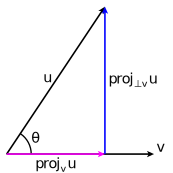
\includegraphics{6_a_Projection.eps}}
\end{center}
\caption{The orthogonal projection of $\vu$ onto $\vv$.}
\label{F:Projection}
\end{figure}

\begin{activity} Since the orthogonal projection $\proj_{\vv} \vu$ is in the direction of $\vv$, there exists a constant $c$ such that $\proj_{\vv} \vu = c \vv$. If we determine the value of  $c$, we can find $\proj_{\vv} \vu$.
\ba 
\item The wind component that acts perpendicular to the direction of $\vv$ is called the projection of $\vu$ orthogonal to $\vv$ and is denoted $\proj_{\perp \vv} \vu$ as shown in Figure \ref{F:Projection}. Write an equation that involves $\proj_{\vv} \vu$, $\proj_{\perp \vv} \vu$, and $\vu$. Then solve that equation for $\proj_{\perp \vv} \vu$. 

\item Given that $\vv$ and $\proj_{\perp \vv} \vu$ are orthogonal, what does that tell us about $\vv \cdot \proj_{\perp \vv} \vu$? Combine this fact with the result of part (a) and that $\proj_{\vv} \vu = c \vv$ to obtain an equation involving $\vv$, $\vu$, and $c$. 

\item Solve for $c$ using the equation you found in the previous step.

\item Use your value of $c$ to identify $\proj_{\vv} \vu$. 
\ea
\end{activity}


To summarize:

\begin{definition} Let $\vu$ and $\vv$ be vectors in $\R^n$ with $\vv \neq \vzero$. 
	\begin{enumerate}
	\item The \textbf{orthogonal projection}\index{orthogonal projection!in the direction of a vector} of $\vu$ onto $\vv$ is the vector 
	\begin{equation}  \label{eq:6_a_projection}
	\proj_{\vv} \vu = \frac{\vu \cdot \vv}{||\vv||^2} \vv.
	\end{equation}
%	\item The \textbf{component}\index{component of one vector in the direction of another} of $\vu$ onto $\vv$ is the scalar
%	\[\comp_{\vv} \vu = \frac{\vu \cdot \vv}{||\vv||}.\]
	\item The \textbf{projection}\index{projection!orthogonal to a vector} of $\vu$ orthogonal to $\vv$ is the vector 
	\[\proj_{\perp \vv} \vu = \vu - \proj_{\vv} \vu.\]
	\end{enumerate}
\end{definition}



\begin{activity} Let $\vu = \left[ \begin{array}{c} 5\\8 \end{array} \right]$ and $\vv = \left[ \begin{array}{r} 6\\-10 \end{array} \right]$. Find $\proj_{\vv} \vu$ and $\proj_{\perp \vv} \vu$ and draw a picture to illustrate.

\end{activity}

The orthogonal projection of a vector $\vu$ onto a vector $\vv$ is really a projection of the vector $\vu$ onto the space $\Span\{\vv\}$. The vector $\proj_{\vv} \vu$ is the best approximation to $\vu$ of all the vectors in $\Span\{\vv\}$ in the sense that $\proj_{\vv} \vu$ is the closest to $\vu$ among all vectors in $\Span\{\vv\}$, as we will prove later.

\csection{Orthogonal Complements}

In Activity \ref{act:6_a_orthogonality} we defined two vectors $\vu$ and $\vv$ in $\R^n$ to be orthogonal (or perpendicular) if $\vu \cdot \vv = 0$. A use of orthogonality in geometry is to define a plane. A plane through the origin in $\R^3$ is a two dimensional subspace of $\R^3$, and a plane is defined to be the set of all vectors in $\R^3$ that are orthogonal to a given vector (called a \emph{normal}\index{normal vector} vector).  For example, to find the equation of the plane through the origin in $\R^3$ orthogonal to the normal vector $\vn = [1 \ 2 \ -1]^{\tr}$, we seek all the vectors $\vv = [x \  y \ z]^{\tr}$ such that
\[\vv \cdot \vn = \vzero.\]
This gives us the equation 
\[x+2y-z = 0\]
as the equation of this plane. The collection of all vectors that are orthogonal to a given subspace of vectors is called the \emph{orthogonal complement} of that subspace in $\R^n$.

\begin{definition} \label{def:6_a_orth_complement} Let $W$ be a subspace of $\R^n$ for some $n \geq 1$. The \textbf{orthogonal complement}\index{orthogonal complement} of $W$ is the set
\[W^{\perp} = \{\vx \in \R^n : \vx \cdot \vw = 0 \text{ for all } \vw \in W\}.\]
\end{definition}

\begin{pa} \label{pa:6_a_2} Let $W = \Span\{[1 \ -1]^{\tr}\}$ in $\R^2$. Completely describe all vectors in $W^{\perp}$ both algebraically and geometrically.

\end{pa}


%orthogonal to the entire space $\Span\{\vv\}$. 


There is a more general idea here as defined in Preview Activity \ref{pa:6_a_2}. If we have a set $S$ of vectors in $\R^n$, we let $S^{\perp}$ (read as ``$S$ perp", called the \emph{orthogonal complement} of $S$) be the set of all vectors in $\R^n$ that are orthogonal to every vector in $S$. In our plane example, the set $S$ is $\{\vn\}$ and $S^{\perp}$ is the plane with equation $x+2y-z=0$.

\begin{activity} We have seen another example of orthogonal complements. Let $A$ be an $m \times n$ matrix with rows $\vr_1$, $\vr_2$ , $\ldots$, $\vr_m$ in order. Consider the three spaces $\Nul A$, $\Row A$, and $\Col A$ related to $A$, where $\Row A = \Span\{\vr_1, \vr_2, \ldots, \vr_m\}$ (that is, $\Row A$ is the span of the rows of $A$). Let $\vx$ be a vector in $\Row A$. 
	\ba
	\item What does it mean for $\vx$ to be in $\Row A$?

	\item Now let $\vy$ be a vector in $\Nul A$. Use the result of part (a) and the fact that $A \vy = \vzero$ to explain why $\vx \cdot \vy = 0$. (Hint: Calculate $A \vy$ using scalar products of rows of $A$ with $\vy$.) Explain how this verifies $(\Row A)^{\perp} = \Nul A$. 

\item Use $A^\tr$ in place of $A$ in the result of the previous part to show $(\Col A)^{\perp} = \Nul A^{\tr}$.
	\ea

\end{activity}

The activity proves the following theorem:

\begin{theorem} \label{thm:6_a_orthogonal_subspaces} Let $A$ be an $m \times n$ matrix. Then
\[(\Row A)^{\perp} = \Nul A \text{ and } (\Col A)^{\perp} = \Nul A^{\tr}.\]
\end{theorem}


To show that a vector is in the orthogonal complement of a subspace, it is not necessary to demonstrate that the vector is orthogonal to every vector in the subspace. If we have a basis for the subspace, it suffices to show that the vector is orthogonal to every vector in that basis for the subspace, as the next theorem demonstrates. 

\begin{theorem} \label{thm:6_a_dot_pd_orth_complement_basis} Let $\CB = \{\vw_1, \vw_2, \ldots, \vw_m\}$ be a basis for a subspace $W$ of $\R^n$. A vector $\vv$ in $\R^n$ is orthogonal to every vector in $W$ if and only if $\vv$ is orthogonal to every vector in $\CB$.
\end{theorem}

\begin{proof} Let $\CB = \{\vw_1, \vw_2, \ldots, \vw_m\}$ be a basis for a subspace $W$ of $\R^n$ and let $\vv$ be a vector in $\R^n$. Our theorem is a biconditional, so we need to prove both implications. Since $\CB \subset W$, it follows that if $\vv$ is orthogonal to every vector in $W$, then $\vv$ is orthogonal to every vector in $\CB$. This proves the forward implication. Now we assume that $\vv$ is orthogonal to every vector in $\CB$ and show that $\vv$ is orthogonal to every vector in $W$. Let $\vx$ be a vector in $W$. Then
\[\vx = x_1\vw_1 + x_2\vw_2 + \cdots + x_m\vw_m\]
for some scalars $x_1$, $x_2$, $\ldots$, $x_m$. Then
\begin{align*}
\vv \cdot \vx &= \vv \cdot (x_1\vw_1 + x_2\vw_2 + \cdots + x_m\vw_m) \\
	&= x_1(\vv \cdot \vw_1) + x_2(\vv \cdot \vw_2) + \cdots + x_m(\vv \cdot \vw_m) \\
	&= 0.
\end{align*}
Thus, $\vv$ is orthogonal to $\vx$ and $\vv$ is orthogonal to every vector in $W$.
\end{proof}

\begin{activity} Let $W = \Span\left\{ \left[ \begin{array}{c} 1 \\ 1 \\ 0 \end{array} \right], \left[ \begin{array}{c} 0 \\ 0 \\ 1 \end{array} \right] \right\}$. Find all vectors in $W^{\perp}$.

\end{activity}

We will work more closely with projections and orthogonal complements in later sections.

\csection{Examples}

\ExampleIntro

\begin{example} Let $\ell$ be the line defined by the equation $ax+by+c=0$ with  in $\R^2$ and let $P = (x_0,y_0)$ be a point in the plane. In this example we will learn how to find the distance from $P$ to $\ell$.  
\ba
\item Show that $\vn = [a \ b]^{\tr}$ is orthogonal to the line $\ell$. That is, $\vn$ is orthogonal to any vector on the line $\ell$. 

\item Let $Q = (x_1, y_1)$ be any point on line $\ell$. Draw a representative picture of $P$, $\vn$ with its initial point at $P$, along with $Q$ and $\ell$.  Explain how to use a projection to determine the distance from $P$ to $\ell$. 

\item Use the idea from part (b) to show that the distance $d$ from $P$ to $\ell$ satisfies
\begin{equation} \label{eq:dist_point_line} 
d = \frac{|ax_0+by_0+c|}{\sqrt{a^2+b^2}}.
\end{equation}

\item Use Equation (\ref{eq:dist_point_line}) to find the distance from the point $(3,4)$ to the line $y = 2x+1$. 

\ea

\ExampleSolution
\ba
\item Any vector on the line $\ell$ is a  vector between two points on the line. Let $Q = (x_1,y_1)$ and $R = (x_2,y_2)$ be points on the line $\ell$. Then $\vu = \overrightarrow{QR} = [x_2-x_1 \ y_2-y_1]^{\tr}$ is a vector on line $\ell$. Since $Q$ and $R$ are on the line, we know that $ax_1+by_1+c=0$ and $ax_2+by_2+c = 0$. So $-c = ax_1+by_1 = ax_2+by_2$ and 
\[0 = a(x_2-x_1) + b(y_2-y_1) = [a \ b]^{\tr} \vu.\]
Thus, $\vn = [a \ b]^{\tr}$ is orthogonal to every vector on the line $\ell$. 

\item A picture of the situation is shown in Figure \ref{F:dist_point_line}. If $\vv = \overrightarrow{PQ}$, then the distance from point $P$ to line $\ell$ is given by $||\proj_{\vn} \vv||$. 
\begin{center}
\begin{figure}[ht] 
\begin{center}
\resizebox{!}{1.5in}{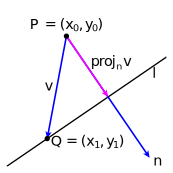
\includegraphics{6_a_distance_line.eps}}
\caption{Distance from a point to a line.}
\label{F:dist_point_line}
\end{center}
\end{figure}
\end{center}

\item Recall that $\vn = [a \ b]^{\tr}$ and $\vv = \overrightarrow{PQ} = [x_1-x_0 \ y_1-y_0]^{\tr}$. Since $ax_1+by_1+c = 0$, we have 
\begin{align*}
\proj_{\vn} \vv &= \frac{\vv \cdot \vv}{||\vn||^2} \vn \\
	&= \frac{a(x_1-x_0)+ b(y_1-y_0)}{a^2+b^2} [a \ b]^{\tr} \\
	&= \frac{ax_1+by_1-ax_0-by_0}{a^2+b^2} [a \ b]^{\tr} \\
	&= \frac{-c-ax_0-by_0}{a^2+b^2} [a \ b]^{\tr}.
\end{align*}
So 
\[||\proj_{\vn} \vv|| = \frac{|ax_0+by_0+c|}{a^2+b^2} \sqrt{a^2+b^2} = \frac{|ax_0+by_0+c|}{\sqrt{a^2+b^2}}.\]

\item Here we have $P = (3,4)$, and the equation of our line is $2x-y+1=0$. So $a=2$, $b=-1$, and $c=-1$. Thus, the distance from $P$ to the line is 
\[\frac{|ax_0+by_0+c|}{\sqrt{a^2+b^2}} = \frac{|2(3)-(4)+1|}{\sqrt{4+1}} = \frac{3}{\sqrt{5}}.\]

\ea

\end{example}

\begin{example} Let $a$, $b$, and $c$ be scalars with $a \neq 0$, and let 
\[W = \{ax+by+cz=0 : x,y,z \in \R\} \, .\]  
\ba
\item Find two vectors that span $W$, showing that $W$ is a subspace of $\R^3$. (In fact, $W$ is a plane through the origin in $\R^3$.)

\item Find a vector $\vn$ that is orthogonal to the two vectors you found in part (a). 

\item Explain why $\{\vn\}$ is a basis for $W^{\perp}$. 

\ea

\ExampleSolution
\ba
\item The coefficient matrix for the system $ax+by+cz = 0$ is $[a \ b \ c]^{\tr}$. The first column is a pivot column and the others are not. So $y$ and $z$ are free variables and 
\[[x \ y \ z]^{\tr} = \left[-\frac{b}{a}y - \frac{c}{a}z, y, z\right]^{\tr} = y\left[ -\frac{b}{a} \ 1 \ 0\right]^{\tr} + z\left[ -\frac{c}{a} \ 0 \ 1\right]^{\tr}.\]
So $W = \Span\left\{\left[ -\frac{b}{a} \ 1 \ 0\right]^{\tr}, \left[ -\frac{c}{a} \ 0 \ 1\right]^{\tr}\right\}$.  

\item If we let $\vn = [a \ b \ c]^{\tr}$, then 
\begin{align*}
\vn \cdot \left[ -\frac{b}{a} \ 1 \ 0\right]^{\tr} &= -b+b = 0 \\
\vn \cdot \left[ -\frac{c}{a} \ 0 \ 1\right]^{\tr}\ &= -c+c = 0.
\end{align*}
Thus, $[a \ b \ c]^{\tr}$ is orthogonal to both $\left[ -\frac{b}{a} \ 1 \ 0\right]^{\tr}$ and $\left[ -\frac{c}{a} \ 0 \ 1\right]^{\tr}$. 

\item Let $\vu = \left[ -\frac{b}{a} \ 1 \ 0\right]^{\tr}$ and $\vv = \left[ -\frac{c}{a} \ 0 \ 1\right]^{\tr}$. Every vector in $W$ has the form $x\vu + y\vv$ for some scalars $x$ and $y$, and 
\[\vn \cdot (x\vu + y\vv) = x(\vn \cdot \vu) + y (\vn \cdot \vv) = 0.\]
So $\vn \in W^{\perp}$. 

Now we need to verify that $\{\vn\}$ spans $W^{\perp}$. Let $\vw = [w_1 \ w_2 \ w_3]^{\tr}$ be in $W^{\perp}$. Then $\vw \cdot \vz = 0$ for every $\vz \in W$. In particular, $\vw \cdot \vu = 0$ or $-\frac{b}{a}w_1 + w_2 = 0$, and $\vw \cdot \vv = 0$ or $-\frac{c}{a}w_1 + w_3 = 0$. Equivalently, we have $w_2 = \frac{b}{a}w_1$ and $w_3 = \frac{c}{a}w_1$. So 
\begin{align*}
\vw &=  [w_1 \ w_2 \ w_3]^{\tr} \\
	&= \left[ w_1 \ \frac{b}{a}w_1 \ \frac{c}{a}w_1\right]^{\tr} \\
	&= \frac{1}{a}[a \ b \ c]^{\tr}w_1 \\
	&= \frac{w_1}{a} \vn.
\end{align*}
So every vector in $W^{\perp}$ is a multiple of $\vn$, and $\{\vn\}$ spans $W^{\perp}$. We conclude that $\{\vn\}$ is a basis for $W^{\perp}$.  Thus, the vector $[a \ b \ c]^{\tr}$ is a normal vector to the plane $ax+by+cz=0$ if $a \neq 0$. The same reasoning works if at least one of $a$, $b$,or $c$ is nonzero, so we can say in every case that $[a \ b \ c]^{\tr}$ is a normal vector to the plane $ax+by+cz=0$.

\ea

\end{example}


\csection{Summary}
\begin{itemize}
\item The dot product of vectors $\vu = [u_1 \ u_2 \  \cdots  \ u_n ]^{\tr}$ and $\vv = [ v_1 \ v_2 \ \cdots \ v_n ]^{\tr}$ in $\R^n$ is the scalar 
\[\vu \cdot \vv = u_1v_1 + u_2v_2 + \cdots + u_nv_n = \displaystyle \sum_{i=1}^n u_iv_i.\]
\item The angle $\theta$ between two nonzero vectors $\vu$ and $\vv$ in $\R^n$ satisfies the equation
\[\cos(\theta) = \frac{\vu \cdot \vv}{||\vu|| \ ||\vv||}\]
and $0\leq \theta \leq 180$.
\item Two vectors $\vu$ and $\vv$ are orthogonal if $\vu \cdot \vv = 0$. 
\item The length, or norm, of the vector $\vu$ can be found as $\ds || \vu || = \sqrt{\vu \cdot \vu}$.
\item The distance between the vectors $\vu$ and $\vv$ in $\R^n$ is $||\vu - \vv ||$, which is the length of the difference $\vu - \vv$.
\item Let $\vu$ and $\vv$ be vectors in $\R^n$. 
	\begin{itemize}
	\item The orthogonal projection of $\vu$ onto $\vv$ is the vector 
	\[\proj_{\vv} \vu = \frac{\vu \cdot \vv}{||\vv||^2} \vv.\]
%	\item The component of $\vu$ onto $\vv$ is the scalar
%	\[\comp_{\vv} \vu = \frac{\vu \cdot \vv}{||\vv||}.\]
	\item The projection of $\vu$ perpendicular to $\vv$ is the vector 
	\[\proj_{\perp \vv} \vu = \vu - \proj_{\vv} \vu.\]
	\end{itemize}
\item The orthogonal complement of the subspace $W$ of $\R^n$ is the set 
\[W^{\perp} = \{\vx \in \R^n : \vx \cdot \vw = 0 \text{ for all } \vw \in W\}.\]
\end{itemize}



\csection{Exercises}
\be
\item For each of the following pairs of vectors, find $\vu \cdot \vv$, calculate the angle between $\vu$ and $\vv$, determine if $\vu$ and $\vv$ are orthogonal, find $||\vu||$ and $||\vv||$, calculate the distance between $\vu$ and $\vv$, and determine the orthogonal  projection of $\vu$ onto $\vv$. 
	\ba
	\item $\vu = [1 \ 2]^{\tr}$, $\vv = [-2 \ 1]^{\tr}$
	\item $\vu = [2 \ -2]^{\tr}$, $\vv = [1 \ -1]^{\tr}$
	\item $\vu = [2 \ -1]^{\tr}$, $\vv = [1 \ 3]^{\tr}$
	\item $\vu = [1 \ 2 \ 0]^{\tr}$, $\vv = [-2 \ 1 \ 1]^{\tr}$
	\item $\vu = [0 \ 0 \ 1]^{\tr}$, $\vv = [1 \ 1 \ 1]^{\tr}$
	\ea

\item Given $\vu=[2 \ 1\ 2]^\tr$, find a vector $\vv$ so that the angle between $\vu$ and $\vv$ is $60^\circ$ and the orthogonal projection of $\vv$ onto $\vu$ has length 2.


\item For which value(s) of $h$ is the angle between $[1\ 1\ h]^\tr$ and $[1\ 2\ 1]^\tr$ equal to $60^\circ$?

\item Let $A = [a_{ij}]$ be a $k \times m$ matrix with rows $\vr_1$, $\vr_2$, $\ldots$, $\vr_k$, and let $B =  [\vb_1 \ \vb_2 \ \cdots \ \vb_n]$ be an $m \times n$ matrix with columns $\vb_1$, $\vb_2$, $\ldots$, $\vb_n$. Show that we can write the matrix product $AB$ in a shorthand way as $AB = [\vr_i \cdot \vb_j]$. 


\item Let $A$ be an $m \times n$, $\vu$ a vector in $\R^n$ and $\vv$ a vector in $\R^m$. Show that 
\[A\vu \cdot \vv = \vu \cdot A^{\tr} \vv.\]


\item Let $\vu$, $\vv$, and $\vw$ be vectors in $\R^n$. Show that 
	\ba
	\item $(\vu + \vv) \cdot \vw = (\vu \cdot \vw) + (\vv \cdot \vw)$ (the dot product \emph{distributes over vector addition})
	\item If $c$ is an arbitrary constant, then $(c\vu) \cdot \vv = \vu \cdot (c\vv) = c(\vu \cdot \vv)$
	\ea

\item \label{ex:Pyth_Thm} The Pythagorean Theorem states that if $a$ and $b$ are the lengths of the legs of a right triangle whose hypotenuse has length $c$, then $a^2+b^2=c^2$. If we think of the legs as defining vectors $\vu$ and $\vv$, then the hypotenuse is the vector $\vu+\vv$ and we can restate the Pythagorean Theorem\index{Pythagorean Theorem in $\R^n$} as 
\[||\vu+\vv||^2 = ||\vu||^2+||\vv||^2.\]
In this exercise we show that this result holds in any dimension.
	\ba
	\item Let $\vu$ and $\vv$ be orthogonal vectors in $\R^n$. Show that $||\vu+\vv||^2 = ||\vu||^2+||\vv||^2$. (Hint: Rewrite $||\vu+\vv||^2$ using the dot product.)  
	\item Must it be true that if $\vu$ and $\vv$ are vectors in $\R^n$ with $||\vu+\vv||^2 = ||\vu||^2+||\vv||^2$, then $\vu$ and $\vv$ are orthogonal? If not, provide a counterexample. If true, verify the statement.
	\ea
	
\item \label{ex:Cauchy_Schwarz} The Cauchy-Schwarz inequality\index{Cauchy-Schwarz inequality!in $\R^n$},
\begin{equation} \label{eq:6_a_Cauchy_Schwartz}
|\vu \cdot \vv| \leq ||\vu|| \ \||\vv||
\end{equation}
for any vectors $\vu$ and $\vv$ in $\R^n$, is considered one of the most important inequalities in mathematics. We verify the Cauchy-Schwarz inequality in this exercise. Let $\vu$ and $\vv$ be vectors in $\R^n$.
	\ba
	\item Explain why the inequality (\ref{eq:6_a_Cauchy_Schwartz}) is true if either $\vu$ or $\vv$ is the zero vector. As a consequence, we assume that $\vu$ and $\vv$ are nonzero vectors for the remainder of this exercise. 
	\item Let $\vw = \proj_{\vv} \vu = \frac{\vu \cdot \vv}{||\vv||^2} \vv$ and let $\vz = \vu - \vw$. We know that $\vw \cdot \vz = 0$. Use Exercise \ref{ex:Pyth_Thm} of this section to show that 
	\[||\vu||^2 \geq ||\vw||^2.\]


	\item Now show that $||\vw||^2 = \frac{|\vu \cdot \vv|^2}{||\vv||^2}$. 

	\item Combine parts (b) and (c) to explain why equation (\ref{eq:6_a_Cauchy_Schwartz}) is true. 
	

	\ea
	
\item Let $\vu$ and $\vv$ be vectors in $\R^n$. Then $\vu$, $\vv$ and $\vu+\vv$ form a triangle. We should then expect that the length of any one side of the triangle is smaller than the sum of the lengths of the other sides (since the straight line distance is the shortest distance between two points). In other words, we expect that 
\begin{equation} \label{eq:6_a_triangle_inequality}
||\vu + \vv|| \leq ||\vu|| + ||\vv||.
\end{equation}
Equation (\ref{eq:6_a_triangle_inequality}) is called the \emph{Triangle Inequality}\index{triangle inequality in $\R^n$}. Use the Cauchy-Schwarz inequality (Exercise \ref{ex:Cauchy_Schwarz}) to prove the triangle inequality.

\item Let $W$ be a subspace of $\R^n$ for some $n$. Show that $W^{\perp}$ is also a subspace of $\R^n$. 

\item Let $W$ be a subspace of $\R^n$. Show that $W$ is a subspace of $(W^\perp)^\perp$.

\item If $W$ is a subspace of $\R^n$ for some $n$, what is $W \cap W^{\perp}$? Verify your answer. 

\item Suppose $W_1\subseteq W_2$ are two subspaces of $\R^n$. Show that $W_2^\perp \subseteq W_1^\perp$.

\item What are $\left(\R^n\right)^{\perp}$ and $\{\vzero\}^{\perp}$ in $\R^n$? Justify your answers. 

\item Label each of the following statements as True or False. Provide justification for your response.
	\ba
	\item \textbf{True/False} The dot product is defined between any two vectors. 
	\item \textbf{True/False} If $\vu$ and $\vv$ are vectors in $\R^n$, then $\vu \cdot \vv$ is another vector in $\R^n$. 
	\item \textbf{True/False} If $\vu$ and $\vv$ are vectors in $\R^n$, then $\vu \cdot \vv$ is always non-negative.
	\item \textbf{True/False} If $\vv$ is a vector in $\R^n$, then $\vv \cdot \vv$ is never negative.
	\item \textbf{True/False} If $\vu$ and $\vv$ are vectors in $\R^n$ and $\vu \cdot \vv = 0$, then $\vu = \vv = \vzero$. 
	\item \textbf{True/False} If $\vv$ is a vector in $\R^n$ and $\vv \cdot \vv = 0$, then $\vv = \vzero$. 
	\item \textbf{True/False} The norm of the sum of vectors is the sum of the norms of the vectors. 
	\item \textbf{True/False} If $\vu$ and $\vv$ are vectors in $\R^n$, then $\proj_{\vv} \vu$ is a vector in the same direction as $\vu$. 
	\item \textbf{True/False} The only subspace $W$ of $\R^n$ for which $W^\perp=\{\vzero\}$ is $W=\R^n$.
	\item \textbf{True/False} If a vector $\vu$ is orthogonal to $\vv_1$ and $\vv_2$, then $\vu$ is also orthogonal to $\vv_1+\vv_2$.
	\item \textbf{True/False} If a vector $\vu$ is orthogonal to $\vv_1$ and $\vv_2$, then $\vu$ is also orthogonal to all linear combinations of $\vv_1$ and $\vv_2$.
	\item \textbf{True/False} If $\vu\neq \vzero$ and $\vv$ are parallel, then the orthogonal projection of $\vv$ onto $\vu$ equals $\vv$.
	\item \textbf{True/False} If $\vu\neq \vzero$ and $\vv$ are orthogonal, then the orthogonal projection of $\vv$ onto $\vu$ equals $\vv$.
	\item \textbf{True/False}	For any vector $\vv$ and $\vu\neq \vzero$, $||\proj_\vu \vv|| \leq ||\vv||$.
	\item \textbf{True/False}	Given an $m\times n$ matrix, $\dim(\Row A)+\dim(\Row A)^\perp = n$.
	\item \textbf{True/False} If $A$ is a square matrix, then the columns of $A$ are orthogonal to the vectors in $\Nul A$. 
	\item \textbf{True/False} The vectors in the null space of an $m \times n$ matrix are orthogonal to vectors in the row space of $A$. 

	\ea
\ee

\csection{Project: Back-Face Culling}

To identify hidden polygons in a surface, we will utilize a technique called \emph{back face culling}\index{back-face culling}. This involves identifying which polygons are back facing and which are front facing relative to the viewer's perspective. The first step is to assign a direction to each polygon in a surface. 

\begin{pactivity} \label{act:bf_normal} Consider the polygon $ABCD$ in Figure \ref{F:Normal_vector}. Since a polygon is flat, every vector in the polygon is perpendicular to a fixed vector (which we call a \emph{normal vector} to the polygon). A normal vector $\vn$ for the polygon $ABCD$ in Figure \ref{F:Normal_vector} is shown. In this activity we learn how to find a normal vector to a polygon.

Let  $\vx = [x_1 \ x_2 \ x_3]^{\tr}$ and $\vy = [y_1 \ y_2 \ y_3]^{\tr}$ be two vectors in $\R^3$. If $\vx$ and $\vy$ are linearly independent, then $\vx$ and $\vy$ determine a polygon as shown in Figure \ref{F:Normal_vector}. Our goal is to find a vector $\vn$ that is orthogonal to both $\vx$ and $\vy$. Let $\vw = [w_1 \ w_2 \ w_3]^{\tr}$ be another vector in $\R^3$ and let $C = \left[ \begin{array}{c} \vw^{\tr} \\ \vx^{\tr} \\ \vy^{\tr} \end{array} \right]$ be the matrix whose rows are $\vw$, $\vx$, and $\vy$. Let $C_{ij}$ be the $ij$th cofactor of $C$, that is $C_{ij}$ is $(-1)^{i+j}$ times the determinant of the submatrix of $C$ obtained by deleting the $i$th row and $j$th column of $C$.  Now define the vector $\vx \times \vy$ as follows:
\[\vx \times \vy = C_{11}\ve_1 + C_{12}\ve_2 + C_{13} \ve_3.\]
The vector $\vx \times \vy$ is called the \emph{cross product}\index{cross product} of the vectors $\vx$ and $\vy$. (Note that the cross product is only defined for vectors in $\R^3$.) We will show that $\vx \times \vy$ is orthogonal to both $\vx$ and $\vy$, making $\vx \times \vy$ a normal vector to the polygon defined by $\vx$ and $\vy$.  
\begin{center}
\begin{figure}[ht] 
\begin{center}
\resizebox{!}{1.5in}{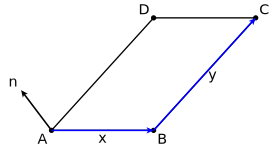
\includegraphics{6_a_normal.eps}}
\caption{Normal vector to a polygon.}
\label{F:Normal_vector}
\end{center}
\end{figure}
\end{center}

\ba
\item Show that 
\[\vx \times \vy = \left[ \begin{array}{c} x_2y_3-x_3y_2 \\ x_3y_1-x_1y_3 \\ x_1y_2-x_2y_1 \end{array} \right].\]


\item  Use a cofactor expansion of $C$ along the first row and properties of the dot product to show that 
\[\det(C) = \vw \cdot (\vx \times \vy).\]


\item Use the result of part (b) and properties of the determinant to calculate $\vx \cdot (\vx \times \vy)$ and $\vy \cdot (\vx \times \vy)$. Explain why $\vx \times \vy$ is orthogonal to both $\vx$ and $\vy$ and is therefore a normal vector to the polygon determined by $\vx$ and $\vy$. 


	\ea
	
\end{pactivity}

Project Activity \ref{act:bf_normal} shows how we can find a normal vector to a parallelogram -- take two vectors $\vx$ and $\vy$ between the vertices of the parallelogram and calculate their cross products. Such a normal vector can define a direction for the parallelogram. There is still a problem, however.

\begin{pactivity} \label{act:bf_normal_2} Let $\vx = [x_1 \ x_2 \ x_3]^{\tr}$ and $\vy = [y_1 \ y_2 \ y_3]^{\tr}$ be any vectors in $\R^3$. There is a relationship between $\vx \times \vy$ and $\vy \times \vx$. Find and verify this relationship.


\end{pactivity}

Project Activity \ref{act:bf_normal_2} shows that the cross product is anticommutative, so we get different directions if we switch the order in which we calculate the cross product. To fix a direction, we establish the convention that we always label the vertices of our parallelogram in the counterclockwise direction as shown in Figure \ref{F:Normal_vector}. This way we always use $\vx$ as the vector from vertex $A$ to vertex $B$ rather than the reverse. With this convention established, we can now define the direction of a parallelogram as the direction of its normal vector.

Once we have a normal vector established for each polygon, we can now determine which polygons are back-face and which are front-face. Figure \ref{F:Hidden} at left provides the gist of the idea, where we represent the polygons with line segments to illustrate. If the viewer's eye is at point $P$ and views the figures, the normal vectors of the visible polygons point in  a direction toward the viewer (front-face) and the normal vectors of the polygons hidden from the viewer point away from the viewer (back-face). What remains is to determine an effective computational way to identify the front and back facing polygons. 

\begin{center}
\begin{figure}[ht] 
\begin{center}
\resizebox{!}{1.25in}{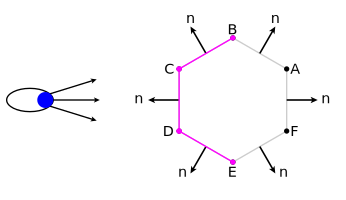
\includegraphics{6_a_hidden.eps}} \hspace{0.5in} 
\resizebox{!}{1.25in}{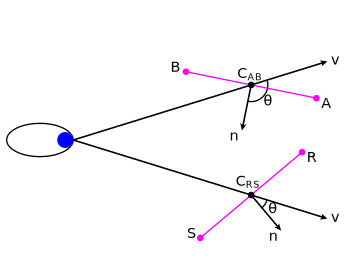
\includegraphics{6_a_cull.eps}}
\caption{Left: Hidden faces. Right: Back face culling.}
\label{F:Hidden}
\end{center}
\end{figure}
\end{center}

\begin{pactivity} \label{act:bf_dot_product} Consider the situation as depicted at right in Figure \ref{F:Hidden}. Assume that $AB$ and $RS$ are polygons (rendered one dimensionally here) with normal vectors $\vn$ at their centers as shown. The viewer's eye is at point $P$ and the viewer's line of vision to the centers $C_{AB}$ and $C_{RS}$ are indicated by the vectors $\vv$. Each vector $\vv$ makes an angle $\theta$ with the normal to the polygon. 
	\ba
	\item What can be said about the angle $\theta$ for a front-facing polygon? What must be true about $\vv \cdot \vn$ for a front-facing polygon? Why?

	
	\item What can be said about the angle $\theta$ for a back-facing polygon? What must be true about $\vv \cdot \vn$ for a back-facing polygon? Why?


	\item The dot product then provides us with a simple computational tool for identifying back-facing polygons (assuming we have already calculated all of the normal vectors). We can then create an algorithm to cull the back-facing polygons. Assuming that we the viewpoint $P$ and the coordinates of the polygons of the surface, complete the pseudo-code for a back-face culling algorithm:

\noindent \textbf{for all} polygons on the surface \textbf{do} \\
\-\hspace{0.25in} 	calculate the normal vector $\vn$ using the \underline{\hspace{0.5in}} product for the current polygon \\
\-\hspace{0.25in} 	calculate the center $C$ of the current polygon \\
\-\hspace{0.25in} 	calculate the viewing vector \underline{\hspace{1in}} \\
\-\hspace{0.5in}	\textbf{if}  \underline{\hspace{1in}} \textbf{then} \\
\-\hspace{0.75in}		render the current polygon \\
\-\hspace{0.5in} 	\textbf{end if} \\
\textbf{end for}
	

	\ea

\end{pactivity} 

As a final comment, back-face culling generally reduces the number of polygons to be rendered by half. This algorithm is not perfect and does not always do what we want it to do (e.g., it may not remove all parts of a polygon that we don't see), so there are other algorithms to use in concert with back-face culling to correctly render objects. 




